% In this section, describe \emph{what you did}. Roughly speaking, explain what data you worked with, how or from where it was collected, 
% it's structure and size. Explain your analysis, and any specific choices you made in it. Depending on the nature of your project, 
% you may focus more or less on certain aspects. If you collected data yourself, explain the collection process in detail. 
% If you downloaded data from the net, show an exploratory analysis that builds intuition for the data, and shows that you know the data well. 
% If you are doing a custom analysis, explain how it works and why it is the right choice. If you are using a standard tool, 
% it may still help to briefly outline it. Cite relevant works. You can use the \verb|\citep| (whole citation in parenthesis) 
% and \verb|\citet| (only year in parenthesis) commands for this purpose \citep{mackay2003information}.

There is no single dataset that contains all the information we need. Thus, we had to combine data from multiple sources. In this section, we will describe the data we used and show exploratory analysis of the data. We will also explain the methods we used to analyze the data.

% SUBSECTION
\subsection{Cardiovascular Diseases data}\label{sec:cardiovascular_data}

The first step in our analysis was to find out whether cardiovascular diseases are an issue in Germany. We used the data from the Global Burden of Disease study \citep{GBD2019} 
to compare the incidence and death rate of cardiovascular diseases in Germany to other high-income countries and the world. The data also contains 
the incidence and death rate for specific age groups which we used to compare the age distribution of cardiovascular diseases in Germany to other countries.
In \figurename~\ref{Cardiovascular diseases over time} we can see that Germany has very high incidence and death rate of cardiovascular diseases. 
\begin{figure*}[h]
    \vskip 0.2in
    \centering
    \centerline{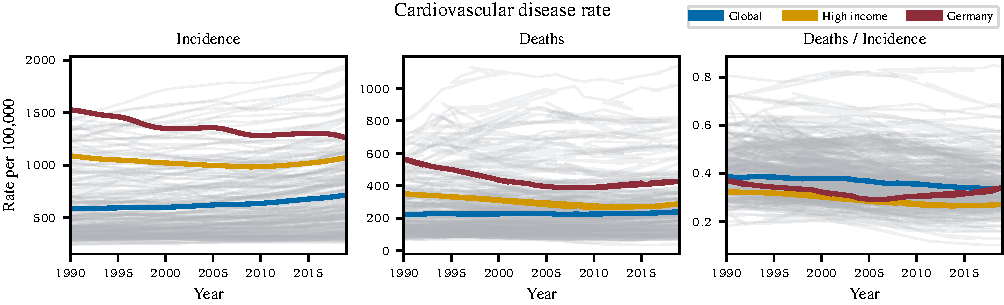
\includegraphics[]{fig/fig_cardiovascular_disease_rate.pdf}}
    \caption{Cardiovascular diseases in the world over time. From left to right: incidence rate, death rate, 
    and the ratio of death rate to incidence rate.}
    \label{Cardiovascular diseases over time}
\end{figure*}

We performed a permutation test to check whether the incidence rate in Germany is statistically significant. In the test, we compared the average incidence rate from 1990 to 2019 of Germany to the average incidence rate of the world. With over a million permutations, we found that the p-value is $\approx 0.045$. When using the standard threshold of 0.05, our p-value would be judged as statistically significant.
In the plot on the right we can also see that the ratio of death rate to incidence rate is much more similar. There appears to be no major difference between the global average and the average of 
high-income countries, which should have a better healthcare system. This suggests that the effect of the quality of healthcare on the ratio is not very significant.

Since cardiovascular diseases are a group of diseases, we wanted to delve deeper and explored the most common cardiovascular diseases in Germany. The top two are ischemic heart disease and stroke (\figurename~\ref{Impact of Different CVDs}). 
We found out that the incidence rate of ischemic heart disease in Germany is also very high, as shown in \href{https://github.com/sykoravojtech/IHD_germany_2024/blob/main/doc/IHD_germany_2024/fig/fig_ischemic_rate.pdf}{its plot}.
The incidence rate of stroke in Germany is way more similar to the global average, as shown in \href{https://github.com/sykoravojtech/IHD_germany_2024/blob/main/doc/IHD_germany_2024/fig/fig_stroke_rate.pdf}{its plot}. This suggests that ischemic heart disease is the main cause of the high incidence rate of cardiovascular diseases in Germany.

\begin{figure}[ht]
    \vskip 0.2in
    \begin{center}
    \centerline{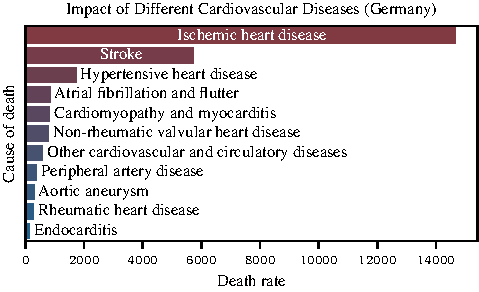
\includegraphics[width=\columnwidth]{fig/fig_ImpactOfDifferentCVDs.pdf}}
    \caption{Death rate of different cardiovascular diseases only for Germany. Ischemic heart disease takes up majority of the deaths.}
    \label{Impact of Different CVDs}
    \end{center}
    \vskip -0.2in
\end{figure}

% SUBSECTION
\subsection{Data sources for factors}\label{sec:data_sources}

Our next step was to use different data sources to find out the underlying factors that have an effect on the incidence rate of ischemic heart disease. We looked at some of the most common risk factors: alcohol consumption and fat consumption. We also included health expenditure as a proxy for the quality of healthcare. Because of the 
distribution of incidence rate depending on age, as shown in \figurename~\ref{Cardiovascular diseases for age groups}, we also included the median age of the population as a factor.

\begin{figure}[ht]
    \vskip 0.2in
    \begin{center}
    \centerline{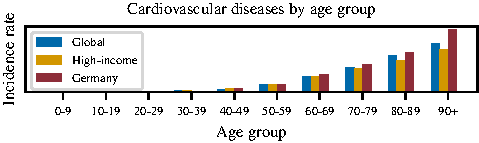
\includegraphics[width=\columnwidth]{fig/fig_cardiovascular_disease_agerange.pdf}}
    \caption{Average incidence rate of cardiovascular diseases for 10 year age groups. The incidence rate is much higher for older age groups, but 
    always the highest in Germany.}
    \label{Cardiovascular diseases for age groups}
    \end{center}
    \vskip -0.2in
\end{figure}

The biggest obstacle was the lack of data that is available for all countries over a long time period. For different factors we had to use different data sources.
The data for health expenditure (as percentage of GDP) and alcohol consumption (liters of pure alcohol per person aged 15 and older) was taken from \citet{oecd}. 
The data for population age is from \citet{age}, while the data for fat consumption (grams per person per day) is from \citet{fat_consumption}. The data varies in the time period it covers,
the number of countries it contains, and the number of missing values, as shown in \tablename~\ref{Data overview}. We used the data from 1990 to 2019, which is the time period
that is available for the diseases.

\begin{table}[h]
    \centering
    \caption{Overview of the data sources. The missing data is calculated for the time period from 1990 to 2019.}
    \label{Data overview}
    \begin{tabular}{|c|c|c|c|}
    \hline
    Data source & No. of countries & Missing data\\
    \hline
    Ischemic heart disease & 206 & 0\%\\
    Health expenditure & 266 & 41\%\\
    Fat consumption & 194 & 0\%\\
    Alcohol consumption & 49 & 0\%\\
    Population age & 238 & 0\%\\
    \hline
    \end{tabular}
\end{table}

\begin{figure*}[ht]
    \vskip 0.2in
    \centering
    \centerline{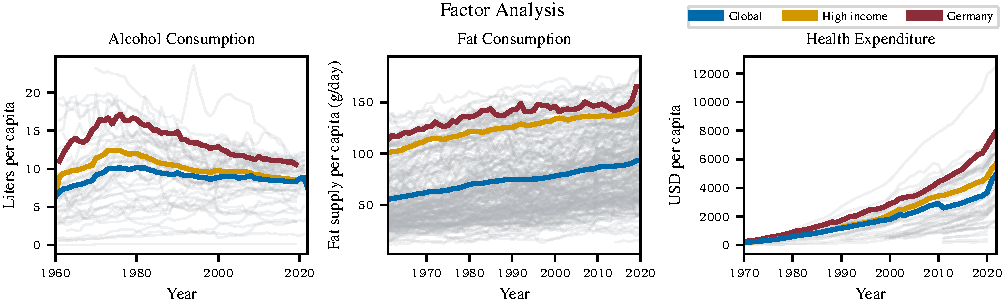
\includegraphics[]{fig/fig_factor_analysis.pdf}}
    \caption{Factor analysis. From left to right: alcohol consumption, fat consumption, and health expenditure. }
    \label{Factor analysis}
\end{figure*}

We made animations and visualizations of the data with enough data points as part of the exploratory analysis. The animations are available at \url{INSERT URL}. 

For the rest of the project we merged the data sources into one dataset, with the goal of modeling the death rate of ischemic heart disease. Because the data sources did not only have different countries, but also different country names we had to do some data preprocessing. The main part was generating ISO-3 country codes for every dataset. 
We decided on not averaging the missing values, but instead filtering them out.

The factors we chose not only reflect the well-known factors of cardiovascular diseases, but also reflect Germany's culture. High alcohol consumption mainly in the form of beer and high fat consumption such as in a Bratwurst are what most of the world knows about this nation. But how out of the ordinary is this behaviour in Germany compared to the rest of the world and other high-income countries? Is Germany's culture pushing them towards a quicker death?

In \figurename~\ref{Factor analysis} in the leftmost plot we can see alcohol consumption per capita in liters. While it has been on a steady decline since the 1970s, Germany still stays far beyond the global and high-income averages. This decline in alcohol consumption is potentially indicative of successful public health interventions, policy reforms, and changing social norms towards alcohol usage within the country. The middle plot presents the trends in fat supply per capita in grams per day. All three highlighted lines show that the trend is gradually increasing while keeping Germany on top. The rightmost plot illustrates health expenditure in USD per capita, where all three cohorts show a substantial increase over the six-decade span.

Alcohol consumption and health spending align with the overarching trend that Germany is trying to diminish the burden from cardiovascular diseases; however, fat consumption seems to go against it. Nevertheless, seeing a difference between two lines does not give a solid view on how each factor truly affects the incidence or death rate which is where the results section comes in.